%%%%%%%%%%%%%%%%%%%%%%%%%%%%%%%%%%%
%This is the LaTeX ARTICLE template for RSC journals
%Copyright The Royal Society of Chemistry 2016
%%%%%%%%%%%%%%%%%%%%%%%%%%%%%%%%%%%

\documentclass[twoside,twocolumn,9pt]{article}
\usepackage{extsizes}
\usepackage[super,sort&compress,comma]{natbib} 
\usepackage[version=3]{mhchem}
\usepackage[left=1.5cm, right=1.5cm, top=1.785cm, bottom=2.0cm]{geometry}
\usepackage{balance}
\usepackage{mathptmx}
\usepackage{sectsty}
\usepackage{graphicx} 
\usepackage{lastpage}
\usepackage[format=plain,justification=justified,singlelinecheck=false,font={stretch=1.125,small,sf},labelfont=bf,labelsep=space]{caption}
\usepackage{float}
\usepackage{fancyhdr}
\usepackage{fnpos}
\usepackage[english]{babel}
\addto{\captionsenglish}{%
  \renewcommand{\refname}{Notes and references}
}
\usepackage{array}
\usepackage{droidsans}
\usepackage{charter}
\usepackage[T1]{fontenc}
\usepackage[usenames,dvipsnames]{xcolor}
\usepackage{setspace}
\usepackage[compact]{titlesec}
\usepackage{hyperref}
%%%Please don't disable any packages in the preamble, as this may cause the template to display incorrectly.%%%


\usepackage{epstopdf}%This line makes .eps figures into .pdf - please comment out if not required.

\definecolor{cream}{RGB}{222,217,201}

\begin{document}

\pagestyle{fancy}
\thispagestyle{plain}
\fancypagestyle{plain}{
%%%HEADER%%%
\renewcommand{\headrulewidth}{0pt}
}
%%%END OF HEADER%%%

%%%PAGE SETUP - Please do not change any commands within this section%%%
\makeFNbottom
\makeatletter
\renewcommand\LARGE{\@setfontsize\LARGE{15pt}{17}}
\renewcommand\Large{\@setfontsize\Large{12pt}{14}}
\renewcommand\large{\@setfontsize\large{10pt}{12}}
\renewcommand\footnotesize{\@setfontsize\footnotesize{7pt}{10}}
\makeatother

\renewcommand{\thefootnote}{\fnsymbol{footnote}}
\renewcommand\footnoterule{\vspace*{1pt}% 
\color{cream}\hrule width 3.5in height 0.4pt \color{black}\vspace*{5pt}} 
\setcounter{secnumdepth}{5}

\makeatletter 
\renewcommand\@biblabel[1]{#1}            
\renewcommand\@makefntext[1]% 
{\noindent\makebox[0pt][r]{\@thefnmark\,}#1}
\makeatother 
\renewcommand{\figurename}{\small{Fig.}~}
\sectionfont{\sffamily\Large}
\subsectionfont{\normalsize}
\subsubsectionfont{\bf}
\setstretch{1.125} %In particular, please do not alter this line.
\setlength{\skip\footins}{0.8cm}
\setlength{\footnotesep}{0.25cm}
\setlength{\jot}{10pt}
\titlespacing*{\section}{0pt}{4pt}{4pt}
\titlespacing*{\subsection}{0pt}{15pt}{1pt}
%%%END OF PAGE SETUP%%%

%%%FOOTER%%%
\fancyfoot{}
\fancyfoot[LO,RE]{\vspace{-7.1pt}
\includegraphics[height=9pt]{head_foot/LF}}
\fancyfoot[CO]{\vspace{-7.1pt}\hspace{13.2cm}
\includegraphics{head_foot/RF}}
\fancyfoot[CE]{\vspace{-7.2pt}\hspace{-14.2cm}
\includegraphics{head_foot/RF}}
\fancyfoot[RO]{\footnotesize{\sffamily{1--\pageref{LastPage} ~\textbar  \hspace{2pt}\thepage}}}
\fancyfoot[LE]{\footnotesize{\sffamily{\thepage~\textbar\hspace{3.45cm} 1--\pageref{LastPage}}}}
\fancyhead{}
\renewcommand{\headrulewidth}{0pt} 
\renewcommand{\footrulewidth}{0pt}
\setlength{\arrayrulewidth}{1pt}
\setlength{\columnsep}{6.5mm}
\setlength\bibsep{1pt}
%%%END OF FOOTER%%%

%%%FIGURE SETUP - please do not change any commands within this section%%%
\makeatletter 
\newlength{\figrulesep} 
\setlength{\figrulesep}{0.5\textfloatsep} 

\newcommand{\topfigrule}{\vspace*{-1pt}% 
\noindent{\color{cream}\rule[-\figrulesep]{\columnwidth}{1.5pt}} }

\newcommand{\botfigrule}{\vspace*{-2pt}% 
\noindent{\color{cream}\rule[\figrulesep]{\columnwidth}{1.5pt}} }

\newcommand{\dblfigrule}{\vspace*{-1pt}% 
\noindent{\color{cream}\rule[-\figrulesep]{\textwidth}{1.5pt}} }

\makeatother
%%%END OF FIGURE SETUP%%%

%%%TITLE, AUTHORS AND ABSTRACT%%%
\twocolumn[
  \begin{@twocolumnfalse}
{
\includegraphics[height=30pt]{head_foot/journal_name}\hfill\raisebox{0pt}[0pt][0pt]{
\includegraphics[height=55pt]{head_foot/RSC_LOGO_CMYK}}\\[1ex]

\includegraphics[width=18.5cm]{head_foot/header_bar}}\par
\vspace{1em}
\sffamily
\begin{tabular}{m{4.5cm} p{13.5cm} }


\includegraphics{head_foot/DOI} & \noindent\LARGE{\textbf{This is the title$^\dag$}} \\%Article title goes here instead of the text "This is the title"
\vspace{0.3cm} & \vspace{0.3cm} \\

 & \noindent\large{Full Name,$^{\ast}$\textit{$^{a}$} Full Name,\textit{$^{b\ddag}$} and Full Name\textit{$^{a}$}} \\%Author names go here instead of "Full name", etc.

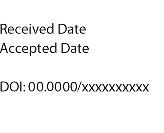
\includegraphics{head_foot/dates} & \noindent\normalsize{The abstract should be a single paragraph which summarises the content of the article. Any references in the abstract should be written out in full \textit{e.g.}\ [Surname \textit{et al., Journal Title}, 2000, \textbf{35}, 3523].} \\%The abstrast goes here instead of the text "The abstract should be..."

\end{tabular}

 \end{@twocolumnfalse} \vspace{0.6cm}

  ]
%%%END OF TITLE, AUTHORS AND ABSTRACT%%%

%%%FONT SETUP - please do not change any commands within this section
\renewcommand*\rmdefault{bch}\normalfont\upshape
\rmfamily
\section*{}
\vspace{-1cm}


%%%FOOTNOTES%%%

\footnotetext{\textit{$^{a}$~Address, Address, Town, Country. Fax: XX XXXX XXXX; Tel: XX XXXX XXXX; E-mail: xxxx@aaa.bbb.ccc}}
\footnotetext{\textit{$^{b}$~Address, Address, Town, Country. }}

%Please use \dag to cite the ESI in the main text of the article.
%If you article does not have ESI please remove the the \dag symbol from the title and the footnotetext below.
\footnotetext{\dag~Electronic Supplementary Information (ESI) available: [details of any supplementary information available should be included here]. See DOI: 00.0000/00000000.}
%additional addresses can be cited as above using the lower-case letters, c, d, e... If all authors are from the same address, no letter is required

\footnotetext{\ddag~Additional footnotes to the title and authors can be included \textit{e.g.}\ `Present address:' or `These authors contributed equally to this work' as above using the symbols: \ddag, \textsection, and \P. Please place the appropriate symbol next to the author's name and include a \texttt{\textbackslash footnotetext} entry in the the correct place in the list.}


%%%END OF FOOTNOTES%%%

%%%MAIN TEXT%%%%
The main text of the article\cite{Mena2000} should appear here.

\subsection{This is the subsection heading style}
Section headings can be typeset with and without numbers.\cite{Abernethy2003}

\subsubsection{This is the subsubsection style.~~} These headings should end in a full point.  

\paragraph{This is the next level heading.~~} For this level please use \texttt{\textbackslash paragraph}. These headings should also end in a full point.

\section{Graphics and tables}
\subsection{Graphics}
Graphics should be inserted on the page where they are first mentioned (unless they are equations, which appear in the flow of the text).\cite{Cotton1999}

\begin{figure}[h]
\centering
  
\includegraphics[height=3cm]{example1}
  \caption{An example figure caption.}
  \label{fgr:example}
\end{figure}

\begin{figure*}
 \centering
 
\includegraphics[height=3cm]{example2}
 \caption{A two-column figure.}
 \label{fgr:example2col}
\end{figure*}

\subsection{Tables}
Tables typeset in RSC house style do not include vertical lines. Table footnote symbols are lower-case italic letters and are typeset at the bottom of the table. Table captions do not end in a full point.\cite{Arduengo1992,Eisenstein2005}


\begin{table}[h]
\small
  \caption{\ An example of a caption to accompany a table}
  \label{tbl:example}
  \begin{tabular*}{0.48\textwidth}{@{\extracolsep{\fill}}lll}
    \hline
    Header one (units) & Header two & Header three \\
    \hline
    1 & 2 & 3 \\
    4 & 5 & 6 \\
    7 & 8 & 9 \\
    10 & 11 & 12 \\
    \hline
  \end{tabular*}
\end{table}

Adding notes to tables can be complicated.  Perhaps the easiest method is to generate these manually.\footnote[4]{Footnotes should appear here. These might include comments relevant to but not central to the matter under discussion, limited experimental and spectral data, and crystallographic data.}

\begin{table*}
\small
  \caption{\ An example of a caption to accompany a table \textendash\ table captions do not end in a full point}
  \label{tbl:example}
  \begin{tabular*}{\textwidth}{@{\extracolsep{\fill}}lllllll}
    \hline
    Header one & Header two & Header three & Header four & Header five & Header six  & Header seven\\
    \hline
    1 & 2 & 3 & 4 & 5 & 6  & 7\\
    8 & 9 & 10 & 11 & 12 & 13 & 14 \\
    15 & 16 & 17 & 18 & 19 & 20 & 21\\
    \hline
  \end{tabular*}
\end{table*}

\section{Equations}

Equations can be typeset inline \textit{e.g.}\ $ y = mx + c$ or displayed with and without numbers:

 \[ A = \pi r^2 \]

\begin{equation}
  \frac{\gamma}{\epsilon x} r^2 = 2r
\end{equation}

You can also put lists into the text. You can have bulleted or numbered lists of almost any kind. 
The \texttt{mhchem} package can also be used so that formulae are easy to input: \texttt{\textbackslash ce\{H2SO4\}} gives \ce{H2SO4}. 

For footnotes in the main text of the article please number the footnotes to avoid duplicate symbols. \textit{e.g.}\ \texttt{\textbackslash footnote[num]\{your text\}}. The corresponding author $\ast$ counts as footnote 1, ESI as footnote 2, \textit{e.g.}\ if there is no ESI, please start at [num]=[2], if ESI is cited in the title please start at [num]=[3] \textit{etc.} Please also cite the ESI within the main body of the text using \dag.

\section{Conclusions}
The conclusions section should come in this section at the end of the article, before the Conflicts of interest statement.

\section*{Conflicts of interest}
In accordance with our policy on \href{http://www.rsc.org/journals-books-databases/journal-authors-reviewers/author-responsibilities/#code-of-conduct}{Conflicts of interest} please ensure that a conflicts of interest statement is included in your manuscript here.  Please note that this statement is required for all submitted manuscripts.  If no conflicts exist, please state that ``There are no conflicts to declare''.

\section*{Acknowledgements}
The Acknowledgements come at the end of an article after Conflicts of interest and before the Notes and references.

%%%END OF MAIN TEXT%%%

%The \balance command can be used to balance the columns on the final page if desired. It should be placed anywhere within the first column of the last page.

\balance

%If notes are included in your references you can change the title from 'References' to 'Notes and references' using the following command:
%\renewcommand\refname{Notes and references}

%%%REFERENCES%%%
\bibliography{rsc} %You need to replace "rsc" on this line with the name of your .bib file
\bibliographystyle{rsc} %the RSC's .bst file

\end{document}
